\section{Contrôle du projet}

\subsection{Statut de l'association}

Rathaxes est une association loi de 1901. Une mise à jour des statuts est
prévue pour fin 2010.

Un compte en banque géré par l'association sera créé afin de subvenir aux
besoins du projet.

Dépenses prévues :
\begin{itemize}
\item Achat de périphériques (souris, carte réseaux, \ldots) ;
\item Voyage (RMLL\footnote{Rencontres Mondiales du Logiciel
Libre(\url{http://rmll.info/}).},
Fosdem\footnote{\url{http://www.fosdem.org/}.}) ;
\item Nom de domaine (rathaxes.org).
\end{itemize}

En tant qu'association, Rathaxes peut recevoir des donations.

\subsection{Environnement de travail}

\begin{itemize}
\item Le LSE est capable de subvenir à la plupart des besoins en matériel ;
\item Trois systèmes d'exploitation seront utilisés pour les recherches et les
tests, trois machines x86 seront donc nécessaires. Cependant elles pourront
être virtualisées afin d'unifier l'environnement de test;
\item Les périphériques de test seront obtenus à partir du LSE ou achetés si
besoin;
\item Le code est hébergé sur GoogleCode à l'adresse :
\url{http://code.google.com/p/rathaxes/} ;
\item Le wiki du google code propose un point de départ pour installer et
tester Rathaxes ;
\item Le code est versionné avec
Mercurial\footnote{\url{http://mercurial.selenic.com/}.} ;
\item Le gestionnaire de bogues (tickets) est public et utilisé pour développer
le projet ;
\item Le code, les tickets ainsi que la documentation doivent être écrits en
anglais ;
\item En plus des courriels EPITECH, chaque membre du projet doit être présent
sur le canal IRC suivant: \url{irc://rathaxes@irc.freenode.org}.
\end{itemize}

\subsection{Planification}

Rathaxes 2012 est la somme de plusieurs étapes :

\begin{enumerate}
\item Étudier des pilotes existant sur chaque plateforme ;
\item Écrire des pilotes sur chaque plateforme ;
\item Définir les concepts à implémenter dans le DSL ;
\item Commencer \`a travailler avec le code de Rathaxes
\item Mettre \`a jour le DSL ;
\item Écrire des pilotes avec Rathaxes ;
\item Participer aux RMLL et Fosdem.
\end{enumerate}

\begin{center}

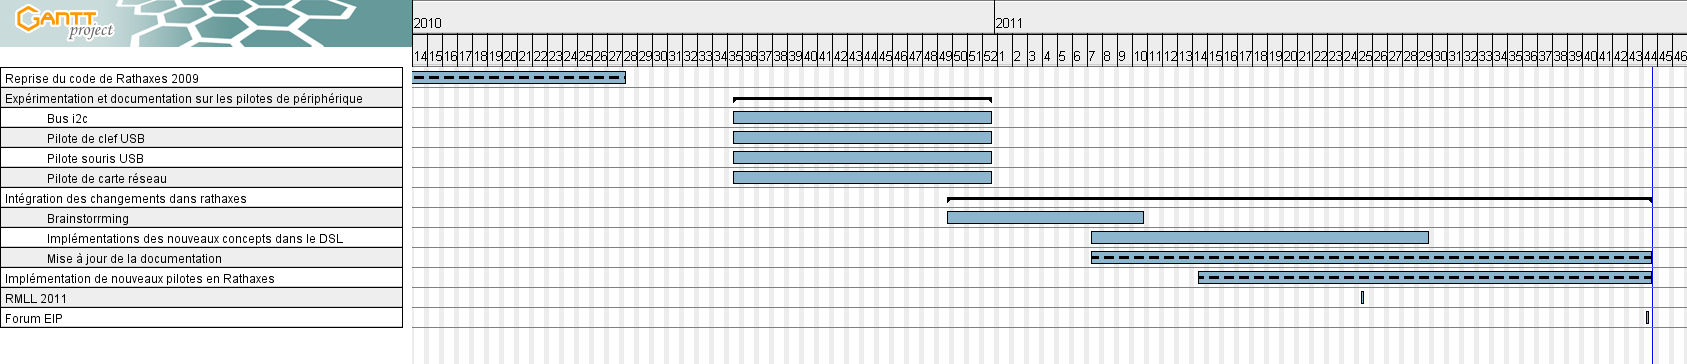
\includegraphics[angle=90,scale=0.35]{../images/gantt}

\end{center}
